\documentclass[twocolumn,a4j]{jsarticle}
\setlength{\topmargin}{-20.4cm}
\setlength{\oddsidemargin}{-10.4mm}
\setlength{\evensidemargin}{-10.4mm}
\setlength{\textwidth}{18cm}
\setlength{\textheight}{26cm}

\usepackage[top=15truemm,bottom=20truemm,left=20truemm,right=20truemm]{geometry}
\usepackage[latin1]{inputenc}
\usepackage{amsmath}
\usepackage{amsfonts}
\usepackage{amssymb}
\usepackage[dvipdfmx]{graphicx}
\usepackage[hang,small,bf]{caption}
\usepackage[subrefformat=parens]{subcaption}
\usepackage[dvipdfmx]{color}
\usepackage{listings}
\usepackage{listings,jvlisting}
\usepackage{geometry}
\usepackage{framed}
\usepackage{color}
\usepackage[dvipdfmx]{hyperref}
\usepackage{ascmac}
\usepackage{enumerate}
\usepackage{tabularx}
\usepackage{cancel}
\usepackage{scalefnt}
\usepackage{overcite}
\usepackage{otf}
\usepackage{multicol}
\usepackage[geometry]{ifsym}
\usepackage{array}

\renewcommand{\figurename}{Fig.}
\renewcommand{\tablename}{Table }

\lstset{
basicstyle={\ttfamily},
identifierstyle={\small},
commentstyle={\smallitshape},
keywordstyle={\small\bfseries},
ndkeywordstyle={\small},
stringstyle={\small\ttfamily},
frame={tb},
breaklines=true,
columns=[l]{fullflexible},
xrightmargin=0zw,
xleftmargin=3zw,
numberstyle={\scriptsize},
stepnumber=1,
numbersep=1zw,
lineskip=-0.5ex
}

% キャプション後ろのダブルコロンを消す
\makeatletter
\long\def\@makecaption#1#2{%
  \vskip\abovecaptionskip
  \iftdir\sbox\@tempboxa{#1\hskip1zw#2}%
    \else\sbox\@tempboxa{#1 #2}%
  \fi
  \ifdim \wd\@tempboxa >\hsize
    \iftdir #1\hskip1zw#2\relax\par
      \else #1 #2\relax\par\fi
  \else
    \global \@minipagefalse
    \hbox to\hsize{\hfil\box\@tempboxa\hfil}%
  \fi
  \vskip\belowcaptionskip}
\makeatother

% タイトル
\makeatletter
\def\@maketitle
{
\begin{center}
{\LARGE \@title \par}
\end{center}
\begin{flushright}
{\large \@date 報告書 No.31}\\
{\large M2 \@author}
\end{flushright}
\par\vskip 1.5em
}
\makeatother

\author{来代 勝胤}
\title{令和4年度 7月 第1週 報告書}
\date{2022/7/4}

\begin{document}
\columnseprule=0.1mm
\maketitle

\section*{報告内容}
\begin{enumerate}[1.]
  \item 数値シミュレーション (粒子数$n_p=1000$)
  \item 来週の予定
\end{enumerate}

\section{数値シミュレーション (粒子数$n_p=1000$)}
数値シミュレーションによる計測手法の精度評価より,
粒子数 $n_p$ -/frame と回転速度 $\omega$ rad/s の関係を調べた.
結果より,本手法における計測精度は $\omega$ より
$n_p$ による影響が大きいことがわかった.
また,$n_p$が大幅に増加した際には内部の処理傾向が
1対1対応の粒子追跡から,パターントラッキングへと移行すると予想される.
そこで,今回は $n_p = 1000$ の場合について数値シミュレーションを行った結果を示す.\\

\subsection{PTVの計算結果とRMSE率}
Fig. 1に,PTVの時間平均結果を示す.
Fig. 1 の結果から,ベクトル抜けが少なく
誤ベクトルの数も少ない.
また,RMSE率の計算結果を Table 1 に示す.
$n_P \leq 500$ の範囲では,$n_p$ の増加に従って
RMSE率も増大していた.
一方で,$n_p = 1000$ のとき,
$n_p = 100$ と同等の計測精度であることがわかる.
したがって,粒子数 $n_p$ が一定以上になると
パターンマッチング領域へと移行し,
計測精度が回復する可能生があると考えられる.

\begin{figure}[htbp]
  \footnotesize
  \begin{center}
    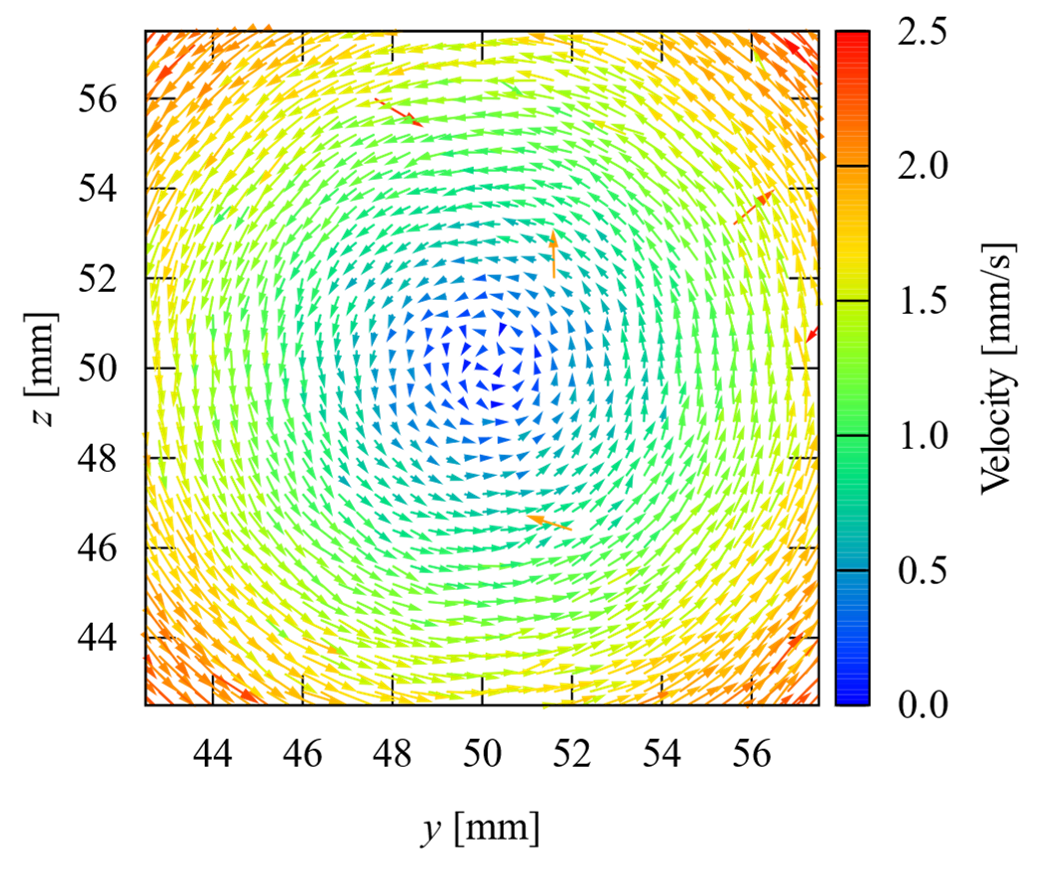
\includegraphics[width=80mm]{../images/velocity_10-1000.png}
    \caption{PTV time-averaged vectors : $n_p = 1000$}
  \end{center}
\end{figure}

\begin{table}[hbtp]
  \centering
  \caption{RMSE ratio : $E$}
  \begin{tabular}{ c c c }
    \hline
    \textgt{$n_p$ [-/frame]} & \textgt{$E$ [\%]} & \\ \hline \hline
    50                       & 2.697             & \\ \hline
    100                      & 3.436             & \\ \hline
    150                      & 4.875             & \\ \hline
    \vdots                   & \vdots            & \\ \hline
    500                      & 5.505             & \\ \hline
    1000                     & 3.059             & \\ \hline
  \end{tabular}
\end{table}

\newpage
また,Table 2にPTVにおける参照領域の面積内に存在する粒子数を
それぞれ
\begin{eqnarray}
  n_b &=& 1.0 + N_p\\
  n_g &=& 1.0 + 3 N_p
\end{eqnarray}
で示す.
これらは,参照領域の面積あたりの粒子数密度 $N_p$ に 1 を足した値になっており,
参照領域を決定する際に,ラベリングプログラムを用いていることから,
ラベリング対象となる1つの粒子と,その周りに存在する粒子数を示すためである.



\begin{table}[hbtp]
  \centering
  \caption{RMSE ratio : $E$}
  \begin{tabular}{ c c c }
    \hline
    \textgt{$n_p$ [-/frame]} & {$n_b$ [-/area]} & {$n_g$ [-/area]} \\ \hline \hline
    50                       & 1.1              & 1.4              \\ \hline
    100                      & 1.3              & 1.8              \\ \hline
    150                      & 1.4              & 2.4              \\ \hline
    \vdots                   & \vdots           & \vdots           \\ \hline
    500                      & 2.4              & 5.2              \\ \hline
    600                      & 2.7              & 6.1              \\ \hline
    700                      & 3.0              & 6.9              \\ \hline
    800                      & 3.3              & 7.8              \\ \hline
    900                      & 3.5              & 8.6              \\ \hline
    1000                     & 3.8              & 9.4              \\ \hline
  \end{tabular}
\end{table}

\section{来週の予定}
\begin{itemize}
  \item 三角翼後流中央部の撮影実験
  \item レンズ変更の影響検証
  \item 粒子追跡プログラムの作成
\end{itemize}

\end{document}